%!TEX root = main.tex
\section{Contenidos del paquete KDSource}

La herramienta KDSource cuenta con los siguiente componentes:
\begin{itemize}
	\item Biblioteca en Python, para estimación de densidad. Aquí se encuentras las herramientas necesarias para crear y optimizar una fuente KDSource en base a una lista de partículas. Se puede además analizar su estadística, generar gráficos de las distribuciones, y exportar la fuente creada, para su uso en los otros componentes de KDSource.
	\item Biblioteca en C, para muestreo. Aquí se encuentras las herramientas necesarias para muestrear nuevas partículas, en base a una fuente KDSource previamente creada.
	\item Aplicación de línea de comando. Permite ejecutar un re-muestreo de partículas, en base a una fuente KDSource previamente creada, obteniéndose una lista de partículas de longitud arbitraria. También permite acceder de forma simple a otras utilidades incuidas en el paquete.
	\item Plantillas y archivos útiles. Facilitan las operaciones más usuales con el paquete KDSource. Se incluyen archivos Jupyter Notebook con las operaciones más usuales de la biblioteca de Python, así como \emph{scripts} y otros componentes para ejecutar algunos códigos Monte Carlo en acople con KDSource.
\end{itemize}

En la Sección \ref{sec:libs} se describen los principales objetos definidos en las librerías, mediante los cuales se modelan y manipulan las fuentes KDE. En los Apéndices  \ref{ap:CLI}, \ref{ap:Python} y \ref{ap:C} se presenta la documentación detallada de la aplicación de línea de comando y de las librerías. Por otra parte, en la Sección \ref{sec:FT} se describe el flujo de trabajo requerido para emplear la herramienta KDSource en una simulación Monte Carlo.


\section{El formato de fuente KDSource}
\label{sec:libs}

La herramienta KDSource cuenta con librerías para modelar fuentes distribucionales de partículas en Python y C. En ambos casos se define la estructura \verb|KDSource|, la cual a su vez posee dos subestructuras: \verb|PList| y \verb|Geometry|. Éstas modelan los dos componentes fundamentales de una fuente KDSource: La lista de partículas y su geometría. En Python, la técnica KDE se implementa a través de la librería \verb|KDEpy| \cite{KDEpy}.

\subsection{Listas de partículas}

Las listas de partículas utilizadas en KDSource utilizan el formato MCPL \cite{MCPL}. El mismo permite la comunicación con los siguientes códigos Monte Carlo:
\begin{itemize}
	\item MCNP
	\item PHITS
	\item McStas
	\item GEANT4
	\item TRIPOLI-4
\end{itemize}
Esto quiere decir que es posible convertir las listas de partículas registradas por cualquiera de estos códigos a MCPL, y viceversa. El \emph{software} asociado al formato MCPL está incluido en la distribución de KDSource, incluyendo funcionalidades extra con respecto a la distribución original, como la posibilidad de comunicación con TRIPOLI-4.

La estructura \verb|PList| empleada en las librerías administra la comunicación con el archivo MCPL. Además de la lectura y escritura, se incluye la posibilidad de aplicar una traslación y rotación a las partículas inmediatamente despues de leerlas, lo cual puede ser útil al acoplar simulaciones con distinto sistema de referencia.

\subsection{Geometría}

A pesar de su nombre, la estructura \verb|Geometry| no sólo administra la geometría de fuente, sino también la manera en que se debe tratar la energía y dirección de las partículas. El objetivo fundamental de esta estructura es convertir el conjunto de parámetros que definen una partícula, es decir energía, posición y dirección, a un vector de parametrización (variables parametrizadas), más adecuado para la aplicación del método KDE. Dicho vector es el que se utilizará como $x$ en las expresiones de la Subsección \ref{subsec:kde}.

Para dar versatilidad al tratamiento energético, espacial y angular deseado, la estructura \verb|Geometry| posee a su vez un conjunto de subestructuras de tipo \verb|Metric|. Usualmente se cuenta con tres de éstas: una para la energía, una para la posición, y una para la dirección. Cada \verb|Metric| define la métrica con la que se tratará cada conjunto de variables. Los objetos \verb|Metric| pueden elegirse del conjunto de métricas implementadas:
\begin{itemize}
	\item \verb|Energy|: tratamiento simple de la energía, sin transformaciones.
	\item \verb|Lethargy|: emplear letargía en lugar de energía.
	\item \verb|Vol|: tratamiento espacial volumétrico.
	\item \verb|SurfXY|: tratamiento espacial plano en XY.
	\item \verb|Guide|: geometría de guía de sección rectangular, con tratamiento de los ángulos basado en la superficie de cada espejo.
	\item \verb|Isotrop|: tratamiento simple de la dirección, basado en el versor unitario de dirección.
	\item \verb|Polar|: tratamiento de la dirección en base a los ángulo $\theta$ (distancia angular a la dirección $\hat{z}$) y $\phi$ (acimut medido desde la dirección $\hat{x}$).
	\item \verb|PolarMu|: igual a \verb|Polar|, pero con $\mu = cos(\theta)$ en lugar de $\theta$.
\end{itemize}

En la biblioteca de Python, la función principal tanto de \verb|Geometry| como de \verb|Metric| es la de transformar las partículas en el formato de partícula de MCPL al vector de parametrización, en formato de \verb|numpy.array|. Esto se logra a través de las funciones \verb|transform| e \verb|inverse_transform|.

En la biblioteca de C, por su parte, considerando que ésta se enfoca en el muestreo de partículas, lo cual se logra mediante la perturbación (ver \ref{subsec:kde}), la función principal de \verb|Geometry| y \verb|Metric| es la de perturbar partículas, respetando la métrica correspondiente y con los anchos de banda provistos. Esto se logra con las funciones \verb|[MetricName]_perturb|, donde \verb|[MetricName]| se debe reemplazar por el nombre de cada métrica.

El objeto \verb|Geometry| también incluye (opcionalmente) una traslación y rotación espacial. Esto permite modelar fuentes ubicadas en dististas posiciones y con distintas orientaciones con respecto al sistema de coordenadas. Por ejemplo, permite modelar una fuente en el plano YZ mediante la métrica \verb|SurfXY|, a través de una rotación de 90 grados en el eje Y. 

\subsection{Archivos de parámetros XML}

Las fuentes creadas en Python, luego de la optimización, pueden guardarse en un archivo de parámetros en formato XML. En el mismo se registran los parámetros que definen las estructuras \verb|PList| y \verb|Geometry| que componen la fuente \verb|KDSource|, así como el \emph{path} al archivo MCPL a utilizar. Este archivo de parámetros puede luego utilizarse para reconstruir la fuente mediante la biblioteca en C, o bien para re-muestrear directamente mediante la aplicación de línea de comando.

Si el ancho de banda del modelo es constante, su valor también se guarda en el mismo archivo XML. Si, por el contrario, el ancho de banda es variable (KDE adaptativo), es decir que se representa con un \emph{array} de un valor por partícula, el mismo se guarda en un archivo separado, en formato binario. Para maximizar el ahorro de memoria, especialmente importante en listas de partículas largas, se utiliza el formato de punto flotante de simple presición (32 bits), sin separación entre valores.


\section{Flujo de trabajo}
\label{sec:FT}

El esquema del flujo de trabajo típico con la herramienta KDSource se esquematiza en la Figura \ref{fig:flujo}. Se parte de una lista de partículas inicial, la cual puede, o no, haber sido creada en una simulación anterior, y luego se ejecuta cierto número de simulaciones Monte Carlo. Cada una de ellas emplea una fuente de partículas KDSource basada en la lista de partículas registrada inmediatamente antes, y registra una nueva lista de partículas para la etapa siguiente. Dependiendo del problema, pueden obtenerse resultados útiles en todas las simulaciones (por ejemplo, al construir un mapa de dosis), o bien sólo en la última (por ejemplo, al calcular el flujo a la salida de un haz). Cada simulación cubre una región de la geometría modelada progresivamente más lejana a la fuente inicial, alcanzando distancias que no serían alcanzables en una sola corrida.

\begin{figure}[b!]
	\centering
	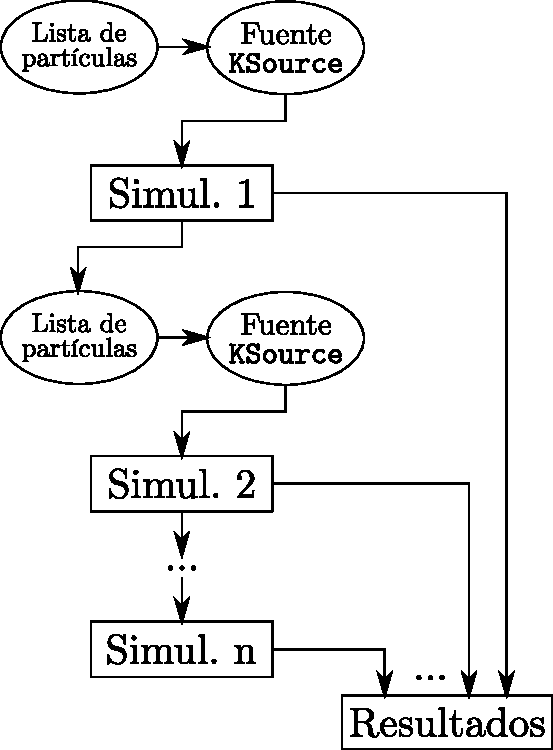
\includegraphics[width=.7\textwidth]{figs/flujo_trabajo.pdf}
	\caption{Esquema del flujo de trabajo típico.}
	\label{fig:flujo}
\end{figure}

Cada construcción de una fuente KDSource en base a una lista de partículas se realiza mediante la API en Python, y culmina al exportar un archivo de parámetros XML. Se provee una plantilla con el código requerido para dicha tarea en el archivo \verb|preproc_tracks.ipynb|.

Es recomendable ejecutar dos veces cada etapa de simulación, una de ellas utilizando la fuente KDE de la manera usual, y en la otra muestreando partículas directamente de la lista de \emph{tracks}. Esto puede lograrse de forma simple fijando el argumento \verb|use_kde=0| en la función de muestreo, empleando la misma fuente \verb|KDSource|. El objetivo de dicha repetición del cálculo es verificar la compatibilidad de los resultados obtenidos con ambas fuentes.

De acuerdo a lo explicado en la Subsección \ref{ssec:KDE-MC}, las fuentes de \emph{tracks} pueden añadir mayor ``ruido'' a la simulación, pero no introducen ningún sesgo. Las fuentes KDE, gracias a su mejor estadística, permiten obtener resultados más detallados en zonas lejanas a la fuente, y más suaves, pero corren el riesgo de introducir errores sistemáticos debidos al sesgo de suavizado. Si los resultados que es posible obtener con ambas simulaciones (cercanos a la fuente) coinciden con ambas fuentes, puede considerarse que el sesgo de la fuente KDE es suficientemente bajo, y ``confiar'' en los resultados más lejanos.


\subsection{Simulaciones con McStas y TRIPOLI-4}

Si el código utilizado fuera McStas o TRIPOLI-4, se incluyen además archivos plantilla para facilitar las tareas de interpretación de los resultados de las simulaciones. El archivo \verb|postproc.ipynb| permite colectar los principales resultados, para su registro en una planilla de cálculo. Por otra parte, el archivo \verb|doseplots.ipynb| facilita la creación de gráficos de los mapas de dosis registrados en TRIPOLI-4, utilizando un módulo de Python incluido para tal fin.


\subsection{Acople entre óptica neutrónica y transporte con McStas}

Entre los componentes de McStas incluidos en el paquete KDSource se encuentra\linebreak \verb|Guide_shielding|, mediante el cual es posible efectuar cálculos de blindaje en la perfiferia de guías neutrónicas, respetando la física correspondiente a la óptica neutrónica. Esto se logra a través de un acople en un solo sentido (\emph{one-way coupling}) entre McStas y un código de transporte de radiación, como MCNP, PHITS o TRIPOLI.

El componente \verb|Guide_shielding|, en una simulación de McStas, funciona de igual manera que otros componentes que simulan guías neutrónicas. En particular modela guías de sección rectangular, con posibilidad de curvatura (similar a \verb|Bender|). La diferencia radica en que, al mismo tiempo que propaga los neutrones en su interior, registra en un archivo MCPL los escapes a través de sus espejos. Es decir que por cada reflexión, se registra la energía, posición y dirección del neutrón incidente, y el peso estadístico de la fracción no reflejada. En McStas la simulación continúa con la porción reflejada.

La lista de partículas obtenida representa una fuente superficial de neutrones escapando a través de los espejos de la guía. Dicha fuente no es plana, sino que tiene forma de tubo, posiblemente curvado, de sección rectangular, y es la causante de la presencia de radiación en la periferia de la guía, la cual debe ser blindada. Este archivo MCPL debe utilizarse entonces para construir una fuente KDE mediante la herramienta KDSource, con ayuda del archivo plantilla \verb|preproc_tracks.ipynb|, y emplear esta última en un cálculo de blindajes de la región que rodea a la guía, tipicamente un búnker o \emph{hall}.

El componente \verb|Guide_shielding| registra, además, las partículas \emph{gamma} emitidas por absorciones en el níquel o titanio de los espejos, de acuerdo a las relaciones presentadas en \cite{abs}. Las absorciones se descuentan del peso estadístico de los neutrones transmitidos, por lo que no afectan las curvas de reflectividad. Por la alta energía de los fotones \emph{prompt} del níquel, el correcto modelado de dicho fenómeno es importante para no subestimar la dosis \emph{gamma} alrededor de la guía, especialmente ante flujos neutrónicos con alta componente térmica y fría. Los fotones generados, con energías obtenidas de los espectros de emisión y direcciones isotrópicamente aleatorias, son registrados en otro archivo MCPL, el cual debe ser utilizado para generar una fuente KDE para un cálculo de blindajes, del mismo modo que con la fuente de escapes neutrónicos.


\subsection{Fuentes de activación con TRIPOLI-4 (u otros códigos)}

Una fuente de activación es una fuente de radiación gamma proveniente del decaimiento radiactivo de nucleidos inestables presentes en un material, producidos mediante reacciones nucleares (activación neutrónica). Dicha fuente no es superficial, sino volumétrica. Desde luego, la herramienta KDSource es capaz de modelar este tipo de fuentes a través de la técnica KDE, pero, como siempre, necesita para ello una lista de partículas. En este caso dicha lista debe contener las propiedades de los fotones al momento de cada decaimiento, cuya interpretación es la siguiente:
\begin{itemize}
	\item Energía: Tiene valores discretos, los cuales, junto con sus frecuencias de ocurrencia, conforman el denominado espectro de decaimiento.
	\item Posición: Se corresponden con los puntos en los que ocurrieron las reacciones de activación.
	\item Dirección: Cada gamma de activación tiene una dirección isotrópicamente aleatoria.
\end{itemize}

Esto quiere decir que, de contarse con una lista de fotones de activación, puede procederse a contruir una fuente KDE con las herramientas descritas anteriormente, en particular con la ayuda del archivo plantilla \verb|preproc_tracks.ipynb|. Debe tenerse la precaución de fijar en cero los anchos de banda en energía, para respetar el carácter discreto del espectro de decaimiento.

Sin embargo, el modo más usual de registrar la activación en materiales es a través de \emph{tallies} volumétricos. En conjunto con el espectro de decaimiento, es posible utilizar dichos \emph{tallies} para crear una lista de gammas de decaimiento, y luego aplicar las herramientas de KDSource. En particular, para el código TRIPOLI-4, la API en Python de KDSource cuenta con un módulo que permite realizar de forma sencilla la conversión de \emph{tally} a lista de \emph{tracks}, mediante la clase \verb|T4Tally|. Además, el archivo plantilla \verb|preproc_tally.ipynb| cuenta con el conjunto de operaciones necesarias para construir una fuente KDE, en base a un \emph{tally} de activación de TRIPOLI-4 y un espectro de decaimiento. 
